%% Elsevier 'elsarticle' template — Structures (review mode)
\pdfminorversion=7 % allow inclusion of up to PDF 1.7 graphics
\documentclass[review,12pt]{elsarticle} % ilk gönderimde review + tek sütun
\journal{Structures}
\biboptions{square}

%% Packages
\usepackage[english]{babel}
\usepackage{amsmath,amssymb,mathtools}
\usepackage{graphicx}
\usepackage{siunitx}
\usepackage{microtype}
% Microtype'ın 2025 sürümünde \microtypecontext için "showhyphens" anahtarı
% kaldırıldığından, yamayı kapatmak için yeni yaklaşıma geçiyoruz.
% lineno ile uyumluluk adına \showhyphens düzeltmesini yalnızca devre dışı bırakıyoruz.
\makeatletter
\AtBeginDocument{%% yeni microtype yamalarını koşullu olarak kapat
\@ifundefined{MT@patch@showhyphens}{}{%% yama mevcutsa
\@ifundefined{DisableMicrotypePatch}{}{%% komut tanımlıysa uygula
\DisableMicrotypePatch{showhyphens}%
}%
}%
}
\makeatother
\usepackage{lineno}
\usepackage{booktabs}
\usepackage{tabularx}
\usepackage{array}
\usepackage{ragged2e} % daha iyi satır sonu için (opsiyonel)
\usepackage{placeins}



%% siunitx
\sisetup{
mode = match,
propagate-math-font = true,
reset-math-version = false,
reset-text-family = false,
reset-text-series = false,
reset-text-shape = false,
text-family-to-math = true,
text-series-to-math = true,
per-mode = symbol,
range-units = single,
range-phrase = --,
exponent-product = \times
}

%% Microtype
\microtypesetup{expansion,protrusion}
\emergencystretch=3em
\allowdisplaybreaks[1]

% --- HYPERREF EN SONDA ---
\usepackage{hyperref}
\makeatletter
\pdfstringdefDisableCommands{%% disable front-matter commands in PDF strings
\def\corref#1{}
\def\cortext#1{}
\def\cnotenum#1{}
\def\@corref#1{}
}
\makeatother
\newcolumntype{L}{>{\RaggedRight\arraybackslash}X}
\providecommand*{\theHpage}{\thepage}

\begin{document}
\pagenumbering{roman}
\renewcommand*{\theHpage}{FR\roman{page}}
\begin{frontmatter}

\title{Hydro--thermal high-fidelity modelling and multi-objective design of fluid viscous dampers}

%% Authors
\author[aff1]{Ad Soyad\corref{cor1}}
\ead{email@kurum.edu.tr}
\cortext[cor1]{Corresponding author.}

\address[aff1]{Bölüm, Kurum, Şehir, Posta Kodu, Türkiye}

%% Abstract
\begin{abstract}
% 150–250 kelime: Amaç; hidrolik–termal FVD modeli (Cd(Re), kavitasyon, μ(T));
% 10-DOF yapısal model ve zaman entegrasyonu; çok-amaçlı GA (⟨IDR⟩, ⟨PFA⟩);
% başlıca bulgular (yüzdesel azaltımlar, güvenlik metrikleri); pratik tasarım ilkeleri.
\end{abstract}

%% Graphical abstract (ayrı PDF/PNG ekleyebilirsin)
\begin{graphicalabstract}
% \includegraphics[width=\linewidth]{figs/graphical_abstract.pdf}
\end{graphicalabstract}

%% Highlights (3–5 madde)
\begin{highlights}
\item Physics-informed fluid viscous damper with Cd(Re), cavitation soft-limit and two-node thermal coupling.
\item 10-DOF shear-frame under PSA-band scaled ground motions; robust time integration.
\item NSGA-II based multi-objective design reduces both IDR and PFA while satisfying hydraulic/thermal safety.
\end{highlights}

%% Keywords
\begin{keyword}
Fluid viscous damper \sep seismic optimization \sep Cd(Re) \sep cavitation \sep thermal coupling \sep NSGA-II
\end{keyword}
\end{frontmatter}

\hypersetup{pageanchor=false}
\clearpage
\pagenumbering{arabic}
\renewcommand*{\theHpage}{MA\arabic{page}}
\hypersetup{pageanchor=true}


%% ---------------- Main text ----------------
\section{Introduction}
The overall methodology used in this study is summarized in Figure~\ref{fig:overall_workflow}.
\begin{figure}[h!]
  \centering
  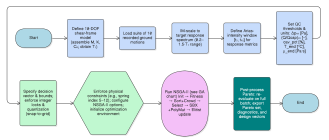
\includegraphics[width=\linewidth]{Genel.pdf} % <-- 1. dosya adınız
  \caption{Overall methodological workflow: (Phase 1) Input Preparation, (Phase 2) GA Setup, and (Phase 3) Optimization Loop.}
  \label{fig:overall_workflow}
\end{figure}
\FloatBarrier
% Motivasyon, literatürde boşluk, katkılar ve makale organizasyonu.

\section{Methods: Physical \& Numerical Modelling}

\begin{sloppypar}
This work utilizes a high-fidelity numerical model coupling the $n$-DOF structural dynamics of a shear frame with the nonlinear hydro-thermal behavior of the FVDs. We intentionally move beyond simplified phenomenological laws (e.g., $F=C|v|^{\alpha}$). Instead, the FVD sub-model is mechanistic [cite: 328], incorporating three critical physical components: (i) orifice hydraulics governed by a Reynolds-dependent discharge coefficient, $C_d(\mathrm{Re})$[cite: 328]; (ii) a physics-based cavitation model employing a smooth pressure limiter [cite: 329]; and (iii) a two-node thermal block that couples fluid temperature directly back to viscosity, $\mu(T)$[cite: 330].
\end{sloppypar}

\par
This integration results in a stiff, coupled ODE system that must advance both structural DOFs and damper temperatures simultaneously[cite: 331]. For numerical robustness and reproducibility, this system is solved using MATLAB's \texttt{ode15s} integrator with strict tolerances ($\text{RelTol}=10^{-3}$ and $\text{AbsTol}=10^{-6}$)[cite: 131, 134, 150, 163]. All performance and safety metrics (PFA, IDR, pressure, temperature) are subsequently evaluated over the significant duration ($t_5-t_{95}$) of the ground motion[cite: 332, 372].

\subsection{Structural model}\label{sec:structural_model}
We idealise the building as a planar, 10-storey \emph{shear-type} frame with one lateral degree of freedom (DOF) per floor. Let $\boldsymbol{x}(t)\!\in\!\mathbb{R}^{10}$ denote \emph{relative} floor displacements (with respect to the moving base) and let $\boldsymbol{r}=\boldsymbol{1}\in\mathbb{R}^{10}$ be the base-excitation influence vector. The equations of motion are
\begin{equation}
  \boldsymbol{M}\,\ddot{\boldsymbol{x}}(t)
  + \boldsymbol{C}_0\,\dot{\boldsymbol{x}}(t)
  + \boldsymbol{K}\,\boldsymbol{x}(t)
  + \boldsymbol{f}_{\mathrm{d}}(t)
  \;=\;
  -\,\boldsymbol{M}\,\boldsymbol{r}\,a_g(t),
  \label{eq:eom}
\end{equation}
where $\boldsymbol{M}$, $\boldsymbol{C}_0$, and $\boldsymbol{K}$ are the mass, structural damping, and stiffness matrices; $\boldsymbol{f}_{\mathrm{d}}(t)$ collects the device-induced nodal forces. All symbols use SI. The full symbol list, assembly details, and the specific parameters for this 10-DOF benchmark structure are consolidated in Appendix~\ref{app:derived}.

\paragraph{Storey kinematics and device coupling}
Let $\boldsymbol{B}\in\mathbb{R}^{9\times 10}$ be the first-difference (incidence) operator, so that storey drift and drift-rate read
\begin{equation}
  \Delta\boldsymbol{x}(t)=\boldsymbol{B}\,\boldsymbol{x}(t),\qquad
  \Delta\dot{\boldsymbol{x}}(t)=\boldsymbol{B}\,\dot{\boldsymbol{x}}(t).
  \label{eq:drift}
\end{equation}
If $\boldsymbol{f}_{\mathrm{story}}(t)\in\mathbb{R}^{9}$ stacks the forces delivered by between-floor devices, the corresponding nodal contribution assembles as
\begin{equation}
  \boldsymbol{f}_{\mathrm{d}}(t)=\boldsymbol{B}^{\mathsf T}\,\boldsymbol{f}_{\mathrm{story}}(t).
  \label{eq:fd_assembly}
\end{equation}

\paragraph{Response measures (Arias window)}
Absolute floor accelerations are
\begin{equation}
  \boldsymbol{a}_{\mathrm{abs}}(t)=\ddot{\boldsymbol{x}}(t)+\boldsymbol{r}\,a_g(t),
  \label{eq:aabs}
\end{equation}
and the roof peak floor acceleration (PFA) is evaluated on the Arias-intensity window $[t_5,t_{95}]$ as
\begin{equation}
  \mathrm{PFA}=\max_{t\in[t_5,t_{95}]}\big|\,\boldsymbol{e}_{10}^{\mathsf T}\boldsymbol{a}_{\mathrm{abs}}(t)\,\big|.
  \label{eq:PFA}
\end{equation}
For uniform storey height $h$, the maximum inter-storey drift ratio (IDR) is
\begin{equation}
  \mathrm{IDR}=\max_{t\in[t_5,t_{95}]}\left\| \frac{\Delta\boldsymbol{x}(t)}{h} \right\|_{\infty}.
  \label{eq:IDR}
\end{equation}

\noindent\textit{Notes.} The standard tri-diagonal assembly of $(\boldsymbol{K},\boldsymbol{C}_0)$ from storey parameters and the modal notation used for intensity scaling (e.g., $T_1$) are deferred to Appendix~\ref{app:derived}; time-domain integration uses Eq.~\eqref{eq:eom} directly.

\subsection{Damper physics}\label{sec:damper_physics}

\begin{figure}[t]
  \centering
  \includegraphics[width=0.9\linewidth]{ViscousDamper_CAD.pdf}
  \caption{Schematic of the high-fidelity fluid viscous damper (FVD) model. Key components include the piston head containing orifices [cite: 1512, 1513] which separates Chamber~1 and Chamber~2 [cite: 1511, 1514], the compressible silicon fluid [cite: 1508], and the parallel spring [cite: 1510] (representing $k_{sd}$).}
  \label{fig:damper_schematic}
\end{figure}

The storey device is modelled as a \emph{parallel} combination of a linear elastic branch and a hydraulic orifice branch, as depicted in Figure~\ref{fig:damper_schematic}. With the storey drift $\Delta x(t)$ and drift rate $\Delta \dot x(t)$ defined as
\begin{equation}
\Delta x(t)=x_{i+1}(t)-x_i(t),\qquad 
\Delta \dot x(t)=\dot x_{i+1}(t)-\dot x_i(t),
\label{eq:dx-dv}
\end{equation}
and with $A_p$ the piston area and $A_o$ the \emph{total} orifice area ($A_o=n_{\mathrm{orf}}\pi d_o^2/4$), the storey force splits into three components:
\begin{equation}
F_{\mathrm{story}}(t)=F_{\mathrm{elastic}}(t)+F_{\mathrm{laminar}}(t)+F_{\mathrm{orifice}}(t),
\label{eq:Fstory}
\end{equation}
where the elastic and laminar contributions are
\begin{equation}
F_{\mathrm{elastic}}(t)=k_{sd}\,\Delta x(t),\qquad
F_{\mathrm{laminar}}(t)=c_{\mathrm{lam}}(T)\,\Delta \dot x(t).
\label{eq:Felam}
\end{equation}
Here $k_{sd}$ lumps the hydraulic/cylinder compliance in series with any coil spring; its full geometric definition is deferred to the Appendix.

\paragraph{Kinematics, layout, and multiplicity}
Positive $\Delta x$ increases the upper chamber volume and decreases the lower one; algebraic flow is taken positive from upper to lower. 

This study models a 2D planar shear-frame, assuming one equivalent damper element ($n_\parallel=1$) is placed at each of the 9 inter-storey levels. The optimization (Section~\ref{sec:opt_ga}) seeks a single, uniform design (i.e., one set of parameters) to be applied to all 9 devices. This $n_\parallel=1$ approach represents the total \emph{equivalent} hydraulic circuit for that storey. In a practical application where multiple physical cylinders are installed in parallel, their contributions (e.g., $A_p$, $A_o$, $hA$) are assumed to be lumped into this single optimized equivalent element, thus avoiding parameter redundancy. For a regular-plan building, the same damper design would be assumed for the orthogonal (Y) direction.

\subsubsection*{Orifice hydraulics: jet loss with $C_d(\mathrm{Re})$ (no linear drop inside $\Delta p$)}
To establish a basis for the safety metric $(Q/Q_{\mathrm{cap}})_{95}$ and to normalize the flow saturation, we first define the theoretical flow capacity, $Q_{\mathrm{cap}}$. This value represents the theoretical maximum flow achievable under a nominal pressure cap, $\Delta p_{\mathrm{cap}}$[cite: 786]. We derive this capacity from the standard orifice equation, assuming fully turbulent conditions ($C_d^\infty$) and a fixed pressure cap (set in the model to $\Delta p_{\mathrm{cap}} = \SI{2e7}{Pa}$, or \SI{20}{MPa})[cite: 788]:
\begin{equation}
Q_{\mathrm{cap}} = C_d^\infty A_o \sqrt{ \frac{2 \Delta p_{\mathrm{cap}}}{\rho(T)} }
\label{eq:Qcap_def}
\end{equation}
This capacity $Q_{\mathrm{cap}}$ then serves as the ceiling for the saturated flow $Q_{\mathrm{sat}}$ used in the jet-loss term, which ensures numerical stability and represents the physical headroom:
\begin{equation}
Q_{\mathrm{sat}}(\Delta\dot x)=
Q_{\mathrm{cap}}\;\tanh\!\Big(\frac{A_p}{Q_{\mathrm{cap}}}\sqrt{\Delta\dot x^{\,2}+v_\varepsilon^{\,2}}\Big),
\qquad v_\varepsilon>0.
\label{eq:Qsat}
\end{equation}
\emph{Only} the quadratic (jet) head loss contributes to the orifice pressure candidate:
\begin{equation}
\Delta p_{\mathrm{kv}}(Q_{\mathrm{sat}},T)=\frac{\rho(T)\,Q_{\mathrm{sat}}\,|Q_{\mathrm{sat}}|}{2\,[C_d(\mathrm{Re})\,A_o]^2},
\label{eq:dp-kv}
\end{equation}
which requires defining the Reynolds number and its corresponding discharge transition:
\begin{equation}
\mathrm{Re}=\frac{\rho(T)\,|Q_{\mathrm{sat}}|\,d_o}{\mu(T)\,A_o},\qquad
C_d(\mathrm{Re})=
C_d^\infty-\frac{C_d^\infty-C_d^0}{1+(\mathrm{Re}/\mathrm{Re}_c)^{p_{\exp}}},
\label{eq:Cd-Re}
\end{equation}
clamped to admissible bounds for $C_d$.

\paragraph{Laminar equivalent (used \emph{outside} $\Delta p_{\mathrm{kv}}$)}
For diagnostics and the explicit viscous branch in Eq.~\eqref{eq:Felam}, the laminar network is represented by its equivalent flow resistance $R_{\mathrm{lam}}$. The resulting laminar coefficient $c_{\mathrm{lam}}$ follows directly from the standard hydraulic-to-mechanical equivalence $c_{\mathrm{lam}} = R_{\mathrm{lam}} A_p^2$:
\begin{equation}
R_{\mathrm{lam}}(T)=\frac{128\,\mu(T)\,L_{\mathrm{ori}}}{\pi\,d_o^4}\,\frac{1}{n_{\mathrm{orf}}},\qquad
c_{\mathrm{lam}}(T)=R_{\mathrm{lam}}(T)\,A_p^2,
\label{eq:Rlam-clam}
\end{equation}
so that $F_{\mathrm{laminar}}=c_{\mathrm{lam}}(T)\,\Delta\dot x$. Note that $R_{\mathrm{lam}}$ does \emph{not} enter Eq.~\eqref{eq:dp-kv}; there is no linear drop inside $\Delta p$.

\subsubsection*{Cavitation limiter (physical model)}\label{sec:damper_cav}
Cavitation is handled by applying a smooth lower bound to the orifice pressure. An upstream pressure proxy follows from the \emph{elastic} term relative to ambient:
\begin{equation}
p_{\uparrow}(t)=p_{\mathrm{amb}}+\frac{|F_{\mathrm{elastic}}(T)|}{A_p}.
\label{eq:pup}
\end{equation}
Comparing $p_{\uparrow}$ to an effective vapour threshold defines the cavitation-limited drop,
\begin{equation}
\Delta p_{\mathrm{cav}}(t)=\max\!\big\{\,\big(p_{\uparrow}(t)-p_{\mathrm{cav,eff}}\big)\cdot \mathrm{cav\_sf},\;0\,\big\},
\label{eq:dpcav}
\end{equation}
and the effective orifice pressure is the differentiable minimum
\begin{equation}
\Delta p_{\mathrm{eff}}=\operatorname{softmin}_{\varepsilon}\!\big(\Delta p_{\mathrm{kv}},\ \Delta p_{\mathrm{cav}}\big).
\label{eq:softmin}
\end{equation}
The cavitation fraction over the Arias window is the time ratio with $\Delta p_{\mathrm{kv}}>\Delta p_{\mathrm{cav}}$.

\paragraph{Orifice force with smoothed sign}
The hydraulic contribution to the storey force is
\begin{equation}
F_{\mathrm{orifice}}(t)=\Delta p_{\mathrm{eff}}(t)\,A_p\,
\frac{\Delta\dot x(t)}{\sqrt{\Delta\dot x^{\,2}(t)+v_\varepsilon^{\,2}}}.
\label{eq:Forf}
\end{equation}

\noindent\textit{Convention.} Linear (laminar) losses act \emph{only} through $c_{\mathrm{lam}}(T)$ in $F_{\mathrm{laminar}}$; the orifice pressure uses the \emph{jet} term with cavitation limiting, i.e. no linear drop is embedded in $\Delta p$.
\subsubsection*{Thermal block (coupled viscosity feedback)}
A compact two-node energy balance (oil $T_o$, steel/cylinder $T_s$) is advanced \emph{concurrently} with the structural state. This ensures that the temperature-dependent viscosity $\mu(T)$ is updated \emph{inside} the force evaluation, feeding back immediately into $c_{\mathrm{lam}}(T)$ and the Reynolds-dependent $C_d(\mathrm{Re}(T))$:
\begin{align}
C_o\,\dot T_o &= P_{\mathrm{loss}} - hA_{o\leftrightarrow s}(T_o-T_s) - hA_{o\leftrightarrow \mathrm{env}}(T_o-T_\infty), \label{eq:To}\\
C_s\,\dot T_s &= \phantom{P_{\mathrm{loss}}}\; +\,hA_{o\leftrightarrow s}(T_o-T_s) - hA_{s\leftrightarrow \mathrm{env}}(T_s-T_\infty). \label{eq:Ts}
\end{align}

\par
To clarify the thermal parameters, we link all three exchange coefficients in Eqs.~\eqref{eq:To}-\eqref{eq:Ts} to the single optimization variable $hA$ (Total thermal conductance) listed in Table~\ref{tab:opt-vars}. We thus assume a lumped parameter model where $hA_{o\leftrightarrow s} = hA_{o\leftrightarrow \mathrm{env}} = hA_{s\leftrightarrow \mathrm{env}} = hA$. This single $hA$ value is varied by the optimizer within its prescribed bounds. The fixed values noted in Appendix Table~\ref{tab:fixed-values-phys} (i.e., \SI{450}{W\,K^{-1}}) correspond to the baseline (non-optimized) configuration only.

\noindent Consistent with the three-term force split, instantaneous mechanical power is the sum of the laminar and orifice contributions (no linear drop inside $\Delta p$):
\begin{equation}
P_{\mathrm{loss}}(t)=
\underbrace{c_{\mathrm{lam}}(T_o)\,\Delta\dot x^{\,2}(t)}_{P_{\mathrm{laminar}}}
+\underbrace{\Delta p_{\mathrm{eff}}(t)\,\big|Q_{\mathrm{sat}}(t)\big|}_{P_{\mathrm{orifice}}}
\;\ge 0 .
\label{eq:Ploss}
\end{equation}
Temperature-dependent properties follow smooth laws:
\begin{equation}
\mu(T)=\mu_{\mathrm{ref}}\,\exp\!\big(b_\mu (T-T_{\mathrm{ref}})\big),\qquad
\rho(T)=\frac{\rho_{\mathrm{ref}}}{1+\alpha_\rho (T-T_{\mathrm{ref}})}.
\label{eq:props}
\end{equation}
The accumulated dissipation reported on the Arias window is
\begin{equation}
E_{\mathrm{mech}}
=\int_{t_5}^{t_{95}} P_{\mathrm{loss}}(t)\,\mathrm{d}t
=\int_{t_5}^{t_{95}} \!\Big(c_{\mathrm{lam}}(T_o)\,\Delta\dot x^{\,2}(t)+\Delta p_{\mathrm{eff}}(t)\,\big|Q_{\mathrm{sat}}(t)\big|\Big)\,\mathrm{d}t .
\label{eq:Emech}
\end{equation}

\paragraph{Parameters (deferred)}
All fixed coefficients, bounds, and geometry for: (i) the discharge-coefficient transition $C_d(\mathrm{Re})$; (ii) damper geometry and elastic/compressibility terms defining $k_{sd}$; (iii) the cavitation limiter; and (iv) thermal exchange and property slopes are consolidated in Appendix~\ref{app:derived} to keep the main text physics-first and reproducible. SI units are used throughout ($Q$ in \si{m^3\,s^{-1}}, $\Delta p$ in \si{Pa}, areas in \si{m^2}).

\subsection{Time integration}\label{sec:time_integration}
We advance the coupled problem with a \emph{stiff, variable–step} ODE scheme. The integrated state collects the structural DOFs and the two–node thermal pair, while damper hydraulics are evaluated \emph{algebraically} inside the right–hand side. With $\boldsymbol{x}(t)\in\mathbb{R}^{10}$ the relative floor displacements and $\boldsymbol{v}(t)=\dot{\boldsymbol{x}}(t)$, the first-order form is:
\[
\boldsymbol{z}(t)=\begin{bmatrix}\boldsymbol{x}(t)\\ \boldsymbol{v}(t)\\ T_o(t)\\ T_s(t)\end{bmatrix},\qquad
\dot{\boldsymbol{x}}=\boldsymbol{v},\qquad
\dot{\boldsymbol{v}}= -\,\boldsymbol{M}^{-1}\!\Big(\boldsymbol{C}_0\,\boldsymbol{v}+\boldsymbol{K}\,\boldsymbol{x}+\boldsymbol{f}_{\mathrm{d}}(t)\Big)\;-\;\boldsymbol{r}\,a_g(t),
\]
where $\boldsymbol{f}_{\mathrm{d}}(t)=\boldsymbol{B}^{\mathsf T}\boldsymbol{f}_{\mathrm{story}}(t)$ and $\boldsymbol{f}_{\mathrm{story}}$ is returned by the mechanistic device model using the instantaneous storey drift rate.

\paragraph{Device evaluation within the RHS}
At each call time, the damper routine uses $\Delta\dot x=\boldsymbol{B}\boldsymbol{v}$ and the current oil temperature to evaluate the saturated flow $Q_{\mathrm{sat}}$ (Eq.~\eqref{eq:Qsat}), the Reynolds number and $C_d(\mathrm{Re})$ (Eq.~\eqref{eq:Cd-Re}), the jet candidate $\Delta p_{\mathrm{kv}}$ (Eq.~\eqref{eq:dp-kv}), and the cavitation–limited $\Delta p_{\mathrm{eff}}$ (Eq.~\eqref{eq:softmin}). The storey force then assembles as the sum of the elastic term, the laminar branch, and the orifice contribution with sign smoothing (Eqs.~\eqref{eq:Felam}, \eqref{eq:Forf}).

\paragraph{Ground motion, integration, and response window}
The base acceleration $a_g(t)$ is accessed via linear interpolation. Given the stiff nature of the coupled system, integration is performed using MATLAB's \texttt{ode15s} solver, enforcing strict tolerances ($\text{RelTol}=10^{-3}$, $\text{AbsTol}=10^{-6}$) for robust reproducibility. The solution is sampled on the native record grid; however, all response metrics are computed only on the Arias–energy window $[t_5,t_{95}]$ to exclude start–up and coda effects.

\paragraph{Thermal coupling}
The two–node thermal block (Eqs.~\eqref{eq:To}–\eqref{eq:Ts}) is advanced concurrently and couples back through $\mu(T_o)$ and $\rho(T_o)$. The mechanical power driving the thermal balance is $P_{\mathrm{loss}}$ in Eq.~\eqref{eq:Ploss}; accumulated dissipation on $[t_5,t_{95}]$ is $E_{\mathrm{mech}}$ in Eq.~\eqref{eq:Emech}.

\paragraph{Initialization and masks}
The structure starts from rest, $\boldsymbol{x}(t_0)=\boldsymbol{0}$ and $\boldsymbol{v}(t_0)=\boldsymbol{0}$. Device multiplicity and storey–activity masks are applied algebraically (areas and linear coefficients scale with $n_\parallel$; inactive storeys are zeroed), preserving sparsity and robustness. Other numerical safeguards (e.g., soft-min sharpness, velocity smoothing) are detailed in Appendix~\ref{app:derived}.

\subsection{Ground Motion Processing and Scaling}
All analyses use a set of 10 recorded horizontal ground motions. Records are converted to SI, de-trended, and may be high-pass filtered (e.g., $f_c{=}0.05$ Hz)[cite: 340].

To ensure a consistent intensity measure (IM) across records, each accelerogram is scaled to a common target $\mathrm{IM}_\star$. This intensity is defined as the band-averaged geometric mean of the 5\%-damped pseudo-spectral acceleration, evaluated on $N$ linearly spaced periods within a band centered on the fundamental period $T_1$, from $T_1/\gamma$ to $\gamma T_1$:
\begin{equation}
\mathrm{IM}_{\mathrm{band}}=\exp\!\left(\frac{1}{N}\sum_{k=1}^{N}\ln S_a^{(5\%)}(T_k)\right), \quad T_k \in [T_1/\gamma,\ \gamma T_1].
\label{eq:IMband}
\end{equation}
The scale factor $s=\mathrm{IM}_\star/\mathrm{IM}_{\mathrm{band}}$, clamped to admissible bounds (e.g., [0.2, 2.2]), is applied to obtain the scaled motion $\tilde a_g(t)$. This scaled motion is then used identically for the bare frame and all damper configurations.

All performance metrics (e.g., PFA, IDR) are evaluated over the significant duration of the motion, defined by the 5\%–95\% Arias-intensity window $[t_5, t_{95}]$, to suppress start-up and coda artefacts[cite: 343]. Per-record metrics are then aggregated (arithmetic means) for the optimization objectives.

\begin{table}[!t]
\centering\footnotesize
\caption{Selected earthquake records used in this study (horizontal components).}
\label{tab:gm-list}
\setlength{\tabcolsep}{6pt}
\renewcommand{\arraystretch}{1.12}
\begin{tabularx}{\linewidth}{@{} 
    l        % Code
    L        % Earthquake name  (esnek, soldan hizalı)
    S[table-format=4.0] % Year
    L        % Station / Component (esnek, soldan hizalı)
    S[table-format=1.1] % Mw
    S[table-format=2.2] % Distance
    S[table-format=1.3] % PGA
@{}}
\toprule
Code & Earthquake name & {Year} & Station / Component & {$M_w$} & {Distance (km)} & {PGA (g)} \\
\midrule
KB95 & Kobe & 1995 & KJMA / KJMA-000                   & 6.9 & 0.96  & 0.833 \\
NR94 & Northridge & 1994 & Sylmar County Hospital / 360 & 6.7 & 9.90  & 0.842 \\
IR80 & Irpinia (Italy) & 1980 & Sturno (STN) / STU270    & 6.9 & 6.78  & 0.320 \\
MJ90 & Manjil & 1990 & Abbar / ABBAR-L                 & 7.3 & 12.55 & 0.510 \\
LP89 & Loma Prieta & 1989 & Calaveras Reservoir / CLR180& 6.9 & 35.28 & 0.110 \\
CC99 & Chi--Chi & 1999 & TCU078 / 90$^\circ$            & 7.6 & 8.30  & 0.442 \\ % 433.6 cm/s^2 → 0.442 g
MR23 & Kahramanmaras (Türkiye) & 2023 & TK~4614 / HNE             & 7.8 & 9.80  & 2.209 \\ % 2166.435 cm/s^2 → 2.209 g
TB78 & Tabas & 1978 & Tabas / H2                        & 7.4 & 2.10  & 0.862 \\
CM92 & Cape Mendocino & 1992 & Petrolia / H2             & 7.0 & 8.20  & 0.662 \\
CH07 & Chuetsu & 2007 & Joetsu Kakizaki / 65010EW      & 6.8 & 9.43  & 0.580 \\
\bottomrule
\end{tabularx}

\vspace{2pt}
{\RaggedRight\footnotesize
Notes: Distances are closest-to-fault (R\textsubscript{rup}) where available. PGA values are in $g$; Chi--Chi and Kahramanmaras are converted from cm/s$^2$ using $1\,g=980.665$ cm/s$^2$ (433.6 $\rightarrow$ 0.442 $g$; 2166.435 $\rightarrow$ 2.209 $g$).
The record set intentionally includes high-PGA, near-fault records (e.g., MR23 at \SI{2.209}{g}) to test the model's robustness. These records are characterized by high-velocity pulses, which impose extreme demands on velocity-dependent devices; their inclusion ensures the optimized design remains safe (in terms of pressure, temperature, and cavitation) even under these severe impulsive loads.
\par}
\end{table}
\FloatBarrier  % <- tablonun bu bölümden aşağı kaymasını engeller

\section{Optimization Framework}\label{sec:opt_ga}

% --- REVİZYON: Metin paragrafı, figürden önceye taşındı ---
We solve a safety-first lexicographic multi-objective problem: designs are ranked by 
$\big[f_{\mathrm{pen}},\, f_1{=}\langle\mathrm{PFA}\rangle,\, f_2{=}\langle\mathrm{IDR}\rangle\big]$; 
we visualise the Pareto trade-off in $(f_1,f_2)$ under $f_{\mathrm{pen}}\!\approx\!0$.
 The goal, illustrated in Figure~\ref{fig:ga_flowchart}, is to identify device parameters $\boldsymbol{d}$ that simultaneously minimize the record-mean roof peak floor acceleration (PFA) and the record-mean maximum inter-storey drift ratio (IDR). These metrics are evaluated over the Arias-window responses $[t_5, t_{95}]$ for a fixed, intensity-scaled set of 10 ground motions.

% --- REVİZYON: Figür, metinden sonraya taşındı ---
\begin{figure}[h!] % <-- [t] yerine [h!] (Here!) kullanıldı
  \centering
  % REVİZYON: Figür, sayfaya sığması için küçültüldü
  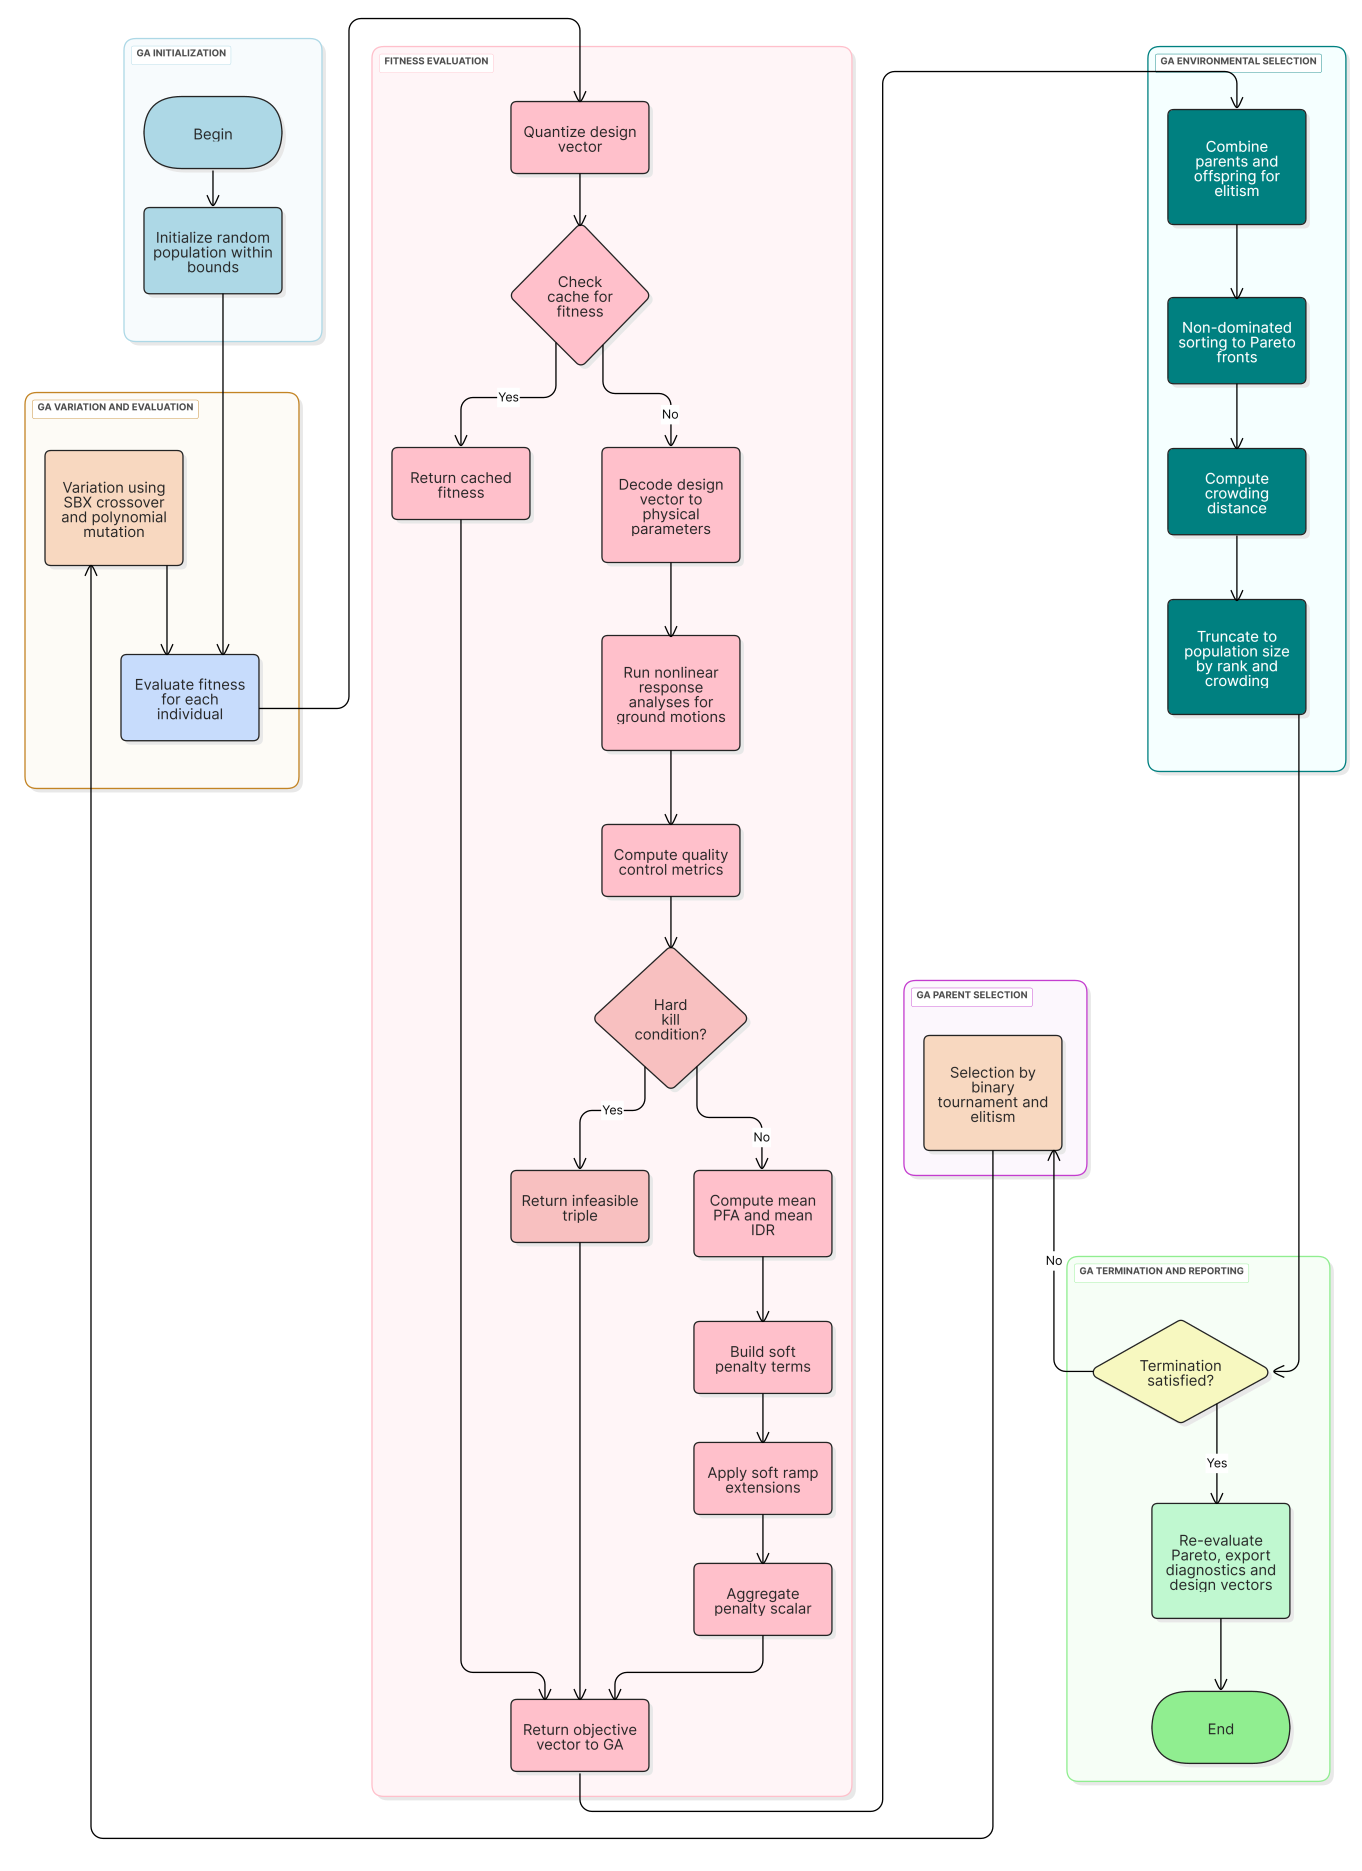
\includegraphics[width=0.75\linewidth]{GA.pdf} % <-- 0.9'dan 0.8'e küçültüldü
  \caption{Flowchart of the NSGA-II optimization process, illustrating population evaluation, safety screening (hard constraints), and multi-objective ranking ($f_{\mathrm{pen}}, f_1, f_2$).}
  \label{fig:ga_flowchart}
\end{figure}

% \FloatBarrier komutu kaldırıldı.

\subsection{Objectives and Safety Constraints}\label{sec:opt_obj}
The primary performance objectives are the record-wise arithmetic means of the structural demands:
\begin{equation}
\min_{\boldsymbol{d}\in\mathcal{X}} \quad
f_1(\boldsymbol{d})=\frac{1}{10}\sum_{j=1}^{10}\mathrm{PFA}_j(\boldsymbol{d}),
\qquad
f_2(\boldsymbol{d})=\frac{1}{10}\sum_{j=1}^{10}\mathrm{IDR}_j(\boldsymbol{d}) ,
\label{eq:obj_main}
\end{equation}
where $\mathcal{X}$ is the admissible (manufacturable and physically valid) design space.

Hydraulic and thermal safety is enforced using a two-tier policy. First, a \emph{hard screen} discards any design that violates the fixed thresholds (see boxed text) on any record. Second, feasible designs are ranked \emph{lexicographically} using the vector:
\[
\big[\,f_{\mathrm{pen}},\; f_1,\; f_2\,\big]
\]
This strategy ensures safety is the primary objective. The penalty function $f_{\mathrm{pen}}$ is a smooth aggregate of normalized safety excesses, which equals zero if all checks are passed and increases monotonically with any near-violation, preserving differentiability for the solver.

\noindent\fbox{%
\parbox{\dimexpr\linewidth-2\fboxsep-2\fboxrule\relax}{%
\textbf{Fixed QC Thresholds (per-record, on Arias window).}
\begin{itemize}
    \item Max. 95th percentile pressure: $\Delta p_{95}\le \SI{4.0e7}{Pa}$
    \item Max. 95th percentile flow ratio: $(Q/Q_{\mathrm{cap}})_{95}\le 0.90$
% --- REVISION START: Cavitation threshold updated ---
    \item Max. cavitation time fraction: $\mathrm{cav}_{\mathrm{pct}} \le 0.5\%$
% --- REVISION END ---
    \item Max. end-of-window temperature: $T_{\mathrm{end}}\le \SI{75}{\celsius}$
    \item Min. end-of-window viscosity: $\mu_{\mathrm{end}}\ge \SI{0.70}{Pa.s}$
\end{itemize}
}}

\par
The safety thresholds defined in the QC box were established conservatively to reflect the operational envelope of industrial FVDs, balancing device longevity, model validity, and material science constraints. These limits are intentionally stringent, aligning with the "safety-first" lexicographic policy.

We justify the primary thresholds as follows:
(i) The internal pressure limit ($\Delta p_{95}\le \SI{4.0e7}{Pa}$, or \SI{40}{MPa}) was selected to ensure mechanical integrity. This provides a significant safety factor against seal extrusion or fatigue, as high-performance damper seals are often rated for pressures up to \SI{275}{MPa}, and typical civil engineering specifications may require burst pressures exceeding \SI{138}{MPa} \cite{TaylorDevices2024}.
(ii) The thermal limits ($T_{\mathrm{end}}\le \SI{75}{\celsius}$ and $\mu_{\mathrm{end}}\ge \SI{0.70}{Pa.s}$) serve a dual purpose. They ensure the device operates within the typical functional range reported in literature (often $-40$ to $+70\,^\circ$C) \cite{MDPI_Thermal2023} and prevent excessive thermal thinning ($\mu_{\mathrm{end}}$) or degradation, which can occur in silicone fluids above \SI{90}{\celsius}. This maintains the validity of the calibrated $\mu(T)$ and $C_d(\mathrm{Re}(T))$ models.
(iii) The flow ratio cap ($(Q/Q_{\mathrm{cap}})_{95}\le 0.90$) imposes a 10\% headroom to prevent the orifice flow from approaching flow saturation (choking), a critical regime where compressibility or cavitation effects can dominate and performance becomes nonlinear \cite{CraneTP410}.
% --- REVISION START: New justification for (iv) ---
(iv) The cavitation policy ($\mathrm{cav}_{\mathrm{pct}} \le 0.5\%$) shifts from a zero-tolerance ideal to a practical, robust threshold designed to be insensitive to spurious numerical noise. To ensure only physically significant events are counted, "cavitation" is defined only when the pressure remains below the effective threshold ($p_{\mathrm{cav,eff}}$) by a \SI{0.5}{kPa} dead-band for a persistent duration ($\tau_{\mathrm{hold}} \ge \SI{5}{ms}$). This \emph{de minimis} 0.5\% time-fraction tolerance ensures that while numerical artifacts are ignored, any design initiating cumulative damage or performance degradation \cite{EN15129_Standard} is still rejected by the hard-screen policy.


Designs breaching any bound are rejected by the hard screen; others are penalized softly via $f_{\mathrm{pen}}$.

\paragraph{Fairness across records.}
To ensure fairness, every candidate design $\boldsymbol{d}$ is evaluated against the \emph{same} set of 10 pre-scaled ground motions and identical modeling/integration policies. No per-record re-tuning is allowed, ensuring objective values reflect only design changes. While the optimization uses means, response dispersion is reported in Section~\ref{sec:results} to support robust engineering choices.

\subsection{Decision Variables and Bounds}\label{sec:opt_vars}
The design vector $\boldsymbol{d}$ collects the 12 key parameters governing the device's hydraulic, elastic, and thermal behavior:
\[
\boldsymbol{d}=\big[
d_o,\ n_{\mathrm{orf}},\ C_d^{0},\ C_d^{\infty},\ p_{\exp},\ L_{\mathrm{ori}},\ hA,\ D_p,\ d_w,\ D_m,\ n_{\mathrm{turn}},\ \mu_{\mathrm{ref}}
\big]^{\mathsf T},
\]
where $d_o$ is the orifice diameter, $n_{\mathrm{orf}}$ the number of parallel orifices (integer), $(C_d^{0},C_d^{\infty},p_{\exp})$ the discharge-law parameters, $L_{\mathrm{ori}}$ the orifice length, $hA$ the total heat-transfer conductance, $(D_p,d_w,D_m,n_{\mathrm{turn}})$ the piston/spring geometry (with $n_{\mathrm{turn}}$ integer), and $\mu_{\mathrm{ref}}$ the reference viscosity.

The feasible region $\mathcal{X}$ is a box-constrained domain (Table~\ref{tab:opt-vars}) with integrality enforced on $n_{\mathrm{orf}}$ and $n_{\mathrm{turn}}$. Bounds are chosen to enforce manufacturability (e.g., minimal drillable $d_o$, feasible spring index $D_m/d_w$) and consistency with the physical models.

\begin{table}[htbp]
  \centering\footnotesize
  \setlength{\tabcolsep}{2pt}
  \caption{Optimization decision variables and bounds.}
  \label{tab:opt-vars}
  \begin{tabularx}{\linewidth}{@{}>{\RaggedRight\arraybackslash}p{0.16\linewidth}%
    >{\RaggedRight\arraybackslash}X%
    >{\centering\arraybackslash}p{0.14\linewidth}%
    >{\centering\arraybackslash}p{0.14\linewidth}%
    >{\RaggedRight\arraybackslash}p{0.18\linewidth}@{}}
  \toprule
  Symbol & Description & {Lower} & {Upper} & Units \\
  \midrule
  $d_o$           & Orifice diameter (per orifice)        & \num{0.00080} & \num{0.00350} & \si{m} \\
  $n_{\mathrm{orf}}$ & Parallel orifices \textit{(integer)}  & \num{3} & \num{12} & -- \\
  $C_d^{0}$       & Discharge coefficient: laminar limit   & \num{0.55} & \num{0.95} & -- \\
  $C_d^{\infty}$  & Discharge coefficient: turbulent limit & \num{0.70} & \num{1.00} & -- \\
  $p_{\exp}$      & $C_d(\mathrm{Re})$ transition exponent & \num{0.90} & \num{1.60} & -- \\
  $L_{\mathrm{ori}}$ & Orifice length                      & \num{0.10} & \num{0.24} & \si{m} \\
  $hA$            & Total thermal conductance              & \num{150} & \num{400} & \si{W\,K^{-1}} \\
  $D_p$           & Piston diameter                        & \num{0.110} & \num{0.260} & \si{m} \\
  $d_w$           & Spring wire diameter                   & \num{0.008} & \num{0.020} & \si{m} \\
  $D_m$           & Spring mean diameter                   & \num{0.080} & \num{0.200} & \si{m} \\
  $n_{\mathrm{turn}}$ & Active spring turns \textit{(integer)} & \num{6} & \num{15} & -- \\
  $\mu_{\mathrm{ref}}$ & Reference viscosity at $T_{\mathrm{ref}}$ & \num{0.60} & \num{2.00} & \si{Pa\,s} \\
  \bottomrule
  \end{tabularx}
  \setlength{\tabcolsep}{6pt}% restore default spacing
\end{table}

\paragraph{Search strategy and audit.}
The bi-objective optimization problem is solved using an elitist, Pareto-based evolutionary solver (NSGA-II class). The algorithm was configured with a population size of 600 and run for 180 generations, utilizing parallel computing to evaluate the full ground-motion set for each candidate design. For robust reproducibility, the search was fixed with a high crossover fraction (`CrossoverFraction=0.90`), Gaussian mutation (`MutationFcn=@mutationgaussian`), and a specific random seed (`rng(42,'twister')`).

After convergence, \emph{each} non-dominated design is re-evaluated to collect extended safety and energy indicators (e.g., pressure percentiles, energy partitions), which are archived and used for the analysis in Section~\ref{sec:results}.

\section{Results and Discussion}\label{sec:results}

This section reports the outcome of the multi-objective optimization and compares the \textbf{Bare Frame} (no dampers) with the \textbf{Optimized System} (the knee-selected FVD from the Pareto front).

\subsection{Evaluation of Seismic Performance Enhancement}
Figures~\ref{fig:top-acc}–\ref{fig:max-idr} compare key Arias-window responses for the Bare Frame and the Optimized System. The optimized design consistently suppresses roof absolute acceleration and inter-storey drift across the record set, indicating that most of the input energy is channelled into damper dissipation rather than structural deformation.

\begin{figure}[t]
  \centering
  \includegraphics[width=0.95\linewidth]{Ust_Kat_Mutlak_Ivme_acc_matrix.pdf}
  \caption{Top–floor absolute acceleration over the Arias window (Bare Frame vs. Optimized FVD).}
  \label{fig:top-acc}
\end{figure}

\begin{figure}[t]
  \centering
  \includegraphics[width=0.95\linewidth]{Ust_Kat_Yer_Degistirme_acc_matrix.pdf}
  \caption{Top–floor displacement over the Arias window (Bare Frame vs. Optimized FVD).}
  \label{fig:top-disp}
\end{figure}

\begin{figure}[t]
  \centering
  \includegraphics[width=0.95\linewidth]{Maksimum_IDR_acc_matrix.pdf}
  \caption{Storey–wise maximum inter–storey drift ratio (Bare Frame vs. Optimized FVD).}
  \label{fig:max-idr}
\end{figure}

The visual trends above are quantified in Table~\ref{tab:perf-summary}. Record-averaged performance is extracted from the post-optimization audit (Section~\ref{sec:opt_ga}): the Baseline row comes from the bare-frame entry, and the Optimized row from the knee-selected design. Relative gains are computed as $100 \times (B-O)/B$.

\begin{table}[htbp]
\centering\small
\caption{Record-averaged performance: Bare Frame vs. knee-selected Optimized FVD (from audit).}
\label{tab:perf-summary}
\begin{tabularx}{\linewidth}{@{}>{\RaggedRight\arraybackslash}X*{4}{>{\centering\arraybackslash}X}@{}}
\toprule
Design & $\overline{\mathrm{PFA}}$ [\si{m/s^2}] & $\overline{\mathrm{IDR}}$ [\%] & $\Delta\mathrm{PFA}$ [\%] & $\Delta\mathrm{IDR}$ [\%]\\
\midrule
Baseline (Bare Frame) & \num{13.27} & \num{0.880} & -- & --\\
Optimized (Knee--FVD)  & \num{5.05}  & \num{0.300} & \num{61.9} & \num{65.9}\\
\bottomrule
\end{tabularx}
\end{table}

\subsection{Multi-Objective Trade-off Analysis and Safety Verification}
Figure~\ref{fig:pareto} displays the final non-dominated set in the objective space $\big(f_1{=}\langle\mathrm{PFA}\rangle,\, f_2{=}\langle\mathrm{IDR}\rangle,\, f_{\mathrm{pen}}\big)$. The proximity of many points to $f_{\mathrm{pen}}\!\approx\!0$ indicates wide feasibility under the strict safety policy defined in Section~\ref{sec:opt_obj}. The knee-selected solution (star) provides a balanced compromise between response mitigation and safety margins.

\par
The knee-selected solution (marked by a star in Figure~\ref{fig:pareto}) was identified using a quantitative compromise programming approach to ensure methodological transparency. First, the search was constrained to the feasible subset of non-dominated solutions that rigorously satisfied the safety-first policy (i.e., $f_{\mathrm{pen}}\!\approx\!0$). Second, the $f_1$ and $f_2$ objectives were normalized using min-max scaling to [0, 1] to prevent bias from their differing units and magnitudes. The 'knee' solution was then defined as the design that minimizes the L2-norm (Euclidean distance) to the normalized utopian point [0, 0], assuming equal weights for both objectives ($w_1=w_2$). This approach provides a robust and repeatable method for selecting a well-balanced compromise solution.

\begin{figure}[t]
\centering
\includegraphics[width=0.82\linewidth]{pareto_front.pdf}
\caption{NSGA–II Pareto front in $(f_1, f_2, f_{\mathrm{pen}})$; star marks the knee–selected design.}
\label{fig:pareto}
\end{figure}

\par
While Table~\ref{tab:perf-summary} presented the record-averaged performance (which served as the optimization objectives), Table~\ref{tab:safety-verification} details the specific safety margins, energy dissipation components, and key peak responses---such as maximum roof displacement and acceleration---for the selected knee-point solution.

\begin{table}[htbp]
\centering\small
\caption{Knee-selected design: detailed safety, energy, and peak response indicators (from re-evaluation audit).}
\label{tab:safety-verification}
\resizebox{\linewidth}{!} & {$T_{\mathrm{end}}$ [\si{\celsius}]} & {$\mu_{\mathrm{end}}$ [\si{Pa.s}]} & {$E_{\mathrm{orifice}}$ [\si{J}]} & {$E_{\mathrm{struct}}$ [\si{J}]} & {$P_{\mathrm{mech}}$ [\si{W}]} & {$E_{\mathrm{ratio}}$}\\
\midrule
Knee–FVD (Xbest) &
0.0517 & 7.6273 &
5.98e6 & 0.634 & 0.00 &
74.1 & 0.70 &
3.52e7 & 2.15e7 & 1.48e6 & 1.63\\
\bottomrule
\end{tabular}}
\end{table}

\begin{table}[htbp]
\centering\small
\caption{Optimized design parameters for the knee-selected FVD (corresponds to Table~\ref{tab:safety-verification}).}
\label{tab:optimized-params}
\begin{tabular}{l l c l}
\toprule
Symbol & Parameter & {Value} & Unit \\
\midrule
$d_o$              & Orifice diameter             & {0.00140} & \si{m} \\
$n_{\mathrm{orf}}$ & Parallel orifices \textit{(int)} & {11}      & -- \\
$C_d^{0}$          & Discharge coeff. (laminar)   & {0.89}    & -- \\
$C_d^{\infty}$     & Discharge coeff. (turbulent) & {0.77}    & -- \\
$p_{\exp}$          & $C_d(\mathrm{Re})$ transition exp. & {1.46}    & -- \\
$L_{\mathrm{ori}}$ & Orifice length               & {0.185}   & \si{m} \\
$hA$               & Total thermal conductance    & {228}     & \si{W\,K^{-1}} \\
$D_p$              & Piston diameter              & {0.157}   & \si{m} \\
$d_w$              & Spring wire diameter         & {0.014}   & \si{m} \\
$D_m$              & Spring mean diameter         & {0.125}   & \si{m} \\
$n_{\mathrm{turn}}$& Active spring turns \textit{(int)}& {10}      & -- \\
$\mu_{\mathrm{ref}}$ & Reference viscosity          & {1.46}    & \si{Pa\,s} \\
\bottomrule
\end{tabular}
\end{table}

\paragraph{Safety verification.}
The knee-selected design, whose parameters are detailed in Table~\ref{tab:optimized-params}, rigorously satisfies all safety constraints defined in Section~\ref{sec:opt_obj}. As confirmed in Table~\ref{tab:safety-verification}, all key metrics remained well within their prescribed limits (e.g., $dP95 < \SI{4.0e7}{Pa}$, $cav\_\% \le 0.00\%$). Notably, the end-of-window viscosity $\mu_{\mathrm{end}} = \SI{0.70}{Pa.s}$ successfully meets the minimum requirement of $\ge \SI{0.70}{Pa.s}$.

\paragraph{Energy dissipation mechanism.}
The re-evaluation confirms the damper's effectiveness. The orifice branch dissipated \SI{3.52e7}{J}, yielding an energy split of $E_{\mathrm{ratio}}=1.63$ relative to structural dissipation (data detailed in Table~\ref{tab:safety-verification}). This confirms the optimized FVDs successfully offload seismic input from the primary structure, explaining the observed reductions in PFA and IDR reported in Table~\ref{tab:perf-summary}.

\paragraph{Summary.}
The safety-first lexicographic search produced a dense, feasible front ($f_{\mathrm{pen}}\!\approx\!0$). The selected knee solution achieved substantial record-averaged reductions in $\langle\mathrm{PFA}\rangle$ and $\langle\mathrm{IDR}\rangle$ (Table~\ref{tab:perf-summary}) while rigorously meeting all pressure, capacity, cavitation, and hydro-thermal safety limits under the fully-coupled model (Table~\ref{tab:safety-verification}).

\section{Conclusions}
% Ana çıkarımlar; mühendislik önerileri; sınırlılıklar ve gelecek çalışmalar.

%% -------------- Back matter --------------
\section*{Data availability}
% Veri/kod erişimi (ör. Zenodo/GitHub bağlantıları).

\section*{CRediT authorship contribution statement}
% ...

\section*{Declaration of competing interest}
% ...

\section*{Acknowledgments}
% ...

%% --- Appendices (place before the bibliography) ---
\appendix
\section{Supplementary symbols and derived quantities}\label{app:derived}
\setcounter{table}{0}
\renewcommand{\thetable}{A.\arabic{table}}
\renewcommand{\theHtable}{A\arabic{table}}

% --- TABLO A.1 ---
\begin{table}[htbp]
\centering\small
\caption{Core structural and coupling symbols (definitions and SI units).}
\label{tab:symbols}
\begin{tabularx}{\linewidth}{@{}>{\RaggedRight\arraybackslash}p{0.18\linewidth}>{\RaggedRight\arraybackslash}p{0.23\linewidth}>{\RaggedRight\arraybackslash}p{0.17\linewidth}>{\RaggedRight\arraybackslash}X@{}}
\toprule
Symbol & Name & Units & Brief definition \\
\midrule
$\boldsymbol{M},\boldsymbol{C}_0,\boldsymbol{K}$ & mass, viscous, stiffness & kg; \si{N.s.m^{-1}}; \si{N.m^{-1}} & Structural operators in Eq.~\eqref{eq:eom}.\\
$\boldsymbol{x},\boldsymbol{v}$ & rel. disp., vel. & m; \si{m.s^{-1}} & Floor DOFs w.r.t. moving base. \\
$\boldsymbol{B}$ & incidence operator & -- & Forms story drifts: $\Delta\boldsymbol{x}=\boldsymbol{B}\boldsymbol{x}$. \\
$\boldsymbol{r}$, $a_g$ & base influence, ground acc. & --; \si{m.s^{-2}} & Base excitation term $-\boldsymbol{M}\boldsymbol{r}a_g$. \\
$A_p, A_o$ & piston, total orifice area & \si{m^2} & $A_p=\pi D_p^2/4$, $A_o=n_{\mathrm{orf}}\pi d_o^2/4$. \\
$\shortstack{$d_o$, $n_{\mathrm{orf}}$,\\ $L_{\mathrm{ori}}$, $D_p$}$ & orifice \& piston geometry & m; --; m; m & Design variables in Table~\ref{tab:opt-vars}. \\
$C_d^0, C_d^\infty, p_{\exp}$ & discharge law params & -- & In $C_d(\mathrm{Re})$. \\
$\mathrm{Re}$ & Reynolds number & -- & $\mathrm{Re}=\rho |Q| d_o/(\mu A_o)$. \\
$k_{sd}$ & elastic branch stiffness & \si{N.m^{-1}} & Series(hydraulic, cylinder) $+$ spring. \\
$c_{\mathrm{lam}}(T)$ & laminar eq. coeff. & \si{N.s.m^{-1}} & Laminar branch (viscous term). \\
\bottomrule
\end{tabularx}
\end{table}

\begin{table}[htbp]
\centering\small
\caption{Core damper and performance symbols (definitions and SI units).}
\label{tab:symbols-damper}
\begin{tabularx}{\linewidth}{@{}>{\RaggedRight\arraybackslash}p{0.18\linewidth}>{\RaggedRight\arraybackslash}p{0.23\linewidth}>{\RaggedRight\arraybackslash}p{0.17\linewidth}>{\RaggedRight\arraybackslash}X@{}}
\toprule
Symbol & Name & Units & Brief definition \\
\midrule
$\Delta p_{\mathrm{kv}}$, $\Delta p_{\mathrm{cav}}$, $\Delta p_{\mathrm{eff}}$ & jet, cavitation, effective drop & Pa & Jet candidate, cavitation cap, soft-min. \\
$Q_{\mathrm{sat}}$, $Q_{\mathrm{cap}}$ & saturated flow, capacity & \si{m^{3}.s^{-1}} & $\tanh$ limiter and capacity. \\
$v_\varepsilon$, $\varepsilon_{\text{softmin}}$ & smoothers & \si{m.s^{-1}}; \si{Pa} & Sign smooth; soft-min sharpness. \\
$\shortstack{$T_o$, $T_s$,\\ $hA$}$ & oil/steel temps., conductance & $^\circ$C; \si{W.K^{-1}} & Two-node thermal block. \\
$\mu(T)$, $\rho(T)$ & viscosity, density & \si{Pa.s}; \si{kg.m^{-3}} & Temperature-dependent properties. \\
$\mathrm{PFA}$, $\mathrm{IDR}$ & peak floor acc., drift ratio & \si{m.s^{-2}}; -- & Main performance metrics. \\
$t_5,t_{95}$ & Arias window bounds & s & Significant duration window for metrics. \\
$P_{\mathrm{loss}}, E_{\mathrm{mech}}$ & mech. power, energy & W; J & Loss split (laminar + jet). \\
\bottomrule
\end{tabularx}
\end{table}

\begin{table}[htbp]
\centering\small
\caption{Structural model parameters (10-DOF shear frame).}
\label{tab:struct-params-appendix}
\begin{tabularx}{\linewidth}{@{}>{\RaggedRight\arraybackslash}p{0.14\linewidth}>{\RaggedRight\arraybackslash}p{0.25\linewidth}>{\RaggedRight\arraybackslash}p{0.18\linewidth}>{\RaggedRight\arraybackslash}p{0.12\linewidth}>{\RaggedRight\arraybackslash}X@{}}
\toprule
Symbol & Name & Value & Units & Notes \\
\midrule
$n$   & number of storeys          & 10                 & --             & One lateral DOF per floor. \\
$m_i$ & storey lumped mass         & \num{3.60e5}       & \si{kg}        & Uniform: $m_i=m$[cite: 824]. \\
$k_i$ & storey lateral stiffness   & \num{6.50e8}       & \si{N/m}       & Uniform: $k_i=k$[cite: 825]. \\
$c_i$ & structural viscous coeff.  & \num{6.20e6}       & \si{N\,s\,m^{-1}} & Uniform: $c_i=c$[cite: 825]. \\
$h$   & storey height              & \num{3.0}          & \si{m}         & Used in Eq.~\eqref{eq:IDR}[cite: 825]. \\
\bottomrule
\end{tabularx}
\end{table}

\begin{table}[htbp]
\centering\scriptsize
\caption{Fixed numeric settings used in this study: optimization QC thresholds and ground-motion parameters.}
\label{tab:fixed-values-qc}
\setlength{\tabcolsep}{3pt}
\begin{tabularx}{\linewidth}{@{}>{\RaggedRight\arraybackslash}p{0.27\linewidth}>{\RaggedRight\arraybackslash}p{0.20\linewidth}>{\RaggedRight\arraybackslash}p{0.16\linewidth}>{\RaggedRight\arraybackslash}X@{}}
\toprule
Symbol & Value & Units & Notes \\
\midrule
\multicolumn{4}{@{}l}{\textit{Optimization QC Thresholds (Section 3.1)}} \\
$\Delta p_{95}^{\max}$ & $4.0\times 10^{7}$ & Pa & QC threshold (per record, windowed). \\
$(Q/Q_{\mathrm{cap}})_{95}^{\max}$ & 0.90 & -- & QC threshold. \\
$\mathrm{cav}^{\max}$ & 0.00 & -- & QC threshold. \\
$T_{\mathrm{end}}^{\max}$ & 75 & $^\circ$C & QC threshold. \\
$\mu_{\mathrm{end}}^{\min}$ & 0.70 & Pa\,s & QC threshold (see Sec.~\ref{sec:opt_obj}). \\
\midrule
\multicolumn{4}{@{}l}{\textit{Ground Motion Parameters (Section 2.4)}} \\
hp\_cut & 0.05 & \si{Hz} & High-pass filter cutoff. \\
band\_fac & [0.8, 1.2] & -- & $T_1$ band factor for IM. \\
band\_N & 21 & -- & Number of periods in the band. \\
s\_bounds & [0.2, 2.2] & -- & Scale factor bounds. \\
\bottomrule
\end{tabularx}
\end{table}

\begin{table}[htbp]
\centering\scriptsize
\caption{Fixed numeric settings used in this study: physical constants for the damper model.}
\label{tab:fixed-values-phys}
\setlength{\tabcolsep}{3pt}
\begin{tabularx}{\linewidth}{@{}>{\RaggedRight\arraybackslash}p{0.27\linewidth}>{\RaggedRight\arraybackslash}p{0.20\linewidth}>{\RaggedRight\arraybackslash}p{0.16\linewidth}>{\RaggedRight\arraybackslash}X@{}}
\toprule
Symbol & Value & Units & Notes \\
\midrule
$p_{\mathrm{cav,eff}}$ & $2.0\times 10^{3}$ & Pa & Cavitation cap. \\
$\mathrm{cav\_sf}$ & 0.90 & -- & Safety factor for cavitation limit. \\
$v_\varepsilon$ & 0.10 & \si{m.s^{-1}} & Sign/flow smoothing. \\
$\varepsilon_{\text{softmin}}$ & $1.0\times 10^{6}$ & Pa & Soft-min sharpness. \\
$T_{\mathrm{ref}}$, $T_\infty$ & 25,\ 25 & $^\circ$C & Viscosity reference \& ambient. \\
$\rho_{\mathrm{ref}}$ & 850 & \si{kg.m^{-3}} & Oil density (ref.). \\
$\mathrm{Re}_c$ & 3000 & -- & Transition Reynolds (in $C_d(\mathrm{Re})$).\\
$p_{\mathrm{amb}}$ & \num{1.0e5} & Pa & Ambient pressure.\\
$K_d$ & \num{1.6e9} & Pa & Bulk modulus proxy (hydraulic stiffness).\\
$L_{\mathrm{gap}}$ & 0.055 & m & Effective chamber length for $k_h, k_s$.\\
$E_{\mathrm{body}}$ & \num{2.1e11} & Pa & Cylinder modulus.\\
$G_{\mathrm{sh}}$ & \num{7.9e10} & Pa & Spring shear modulus.\\
$b_\mu$ & -0.013 & \si{K^{-1}} & Viscosity slope ($\mu(T)$).\\
$\alpha_\rho$ & \textit{[not specified]} & \si{K^{-1}} & Density slope ($\rho(T)$).\\
$C_o,\,C_s$ & \textit{[derived]} & \si{J.K^{-1}} & Thermal capacitances (from $m_{oil}, c_p$).\\
$hA_{o\leftrightarrow s}$ & 450 & \si{W.K^{-1}} & Oil–steel exchange.\\
$hA_{o\leftrightarrow \mathrm{env}}$ & 450 & \si{W.K^{-1}} & Oil–ambient exchange (assumed). \\
$hA_{s\leftrightarrow \mathrm{env}}$ & 450 & \si{W.K^{-1}} & Steel–ambient exchange (assumed). \\
$c_p$ (oil) & 1800 & \si{J.(kg.K)^{-1}} & Specific heat capacity (oil).\\
$c_p$ (steel) & 500 & \si{J.(kg.K)^{-1}} & Specific heat capacity (steel).\\
\bottomrule
\end{tabularx}
\end{table}

% --- TABLO A.4 (Yeniden numaralandırıldı) ---
\begin{table}[htbp]
\centering\footnotesize
\setlength{\tabcolsep}{4.5pt}
\caption{Derived quantities used internally (definitions).}
\label{tab:derived}
\begin{tabularx}{\linewidth}{@{}l>{\RaggedRight\arraybackslash}p{0.32\linewidth}>{\RaggedRight\arraybackslash}X@{}}
\toprule
Quantity & Definition & Role \\
\midrule
$A_p$        & $\pi D_p^2/4$               & Piston area (force $=A_p\,\Delta p$). \\
$A_o$        & $n_{\mathrm{orf}}\pi d_o^2/4$ & Total orifice area. \\
$R_{\mathrm{lam}}$ & Eq.~\eqref{eq:Rlam-clam}  & Laminar head loss term. \\
$C_d(\mathrm{Re})$ & Eq.~\eqref{eq:Cd-Re}     & Discharge coefficient. \\
$k_h$        & $K_d A_p^2/L_{\mathrm{gap}}$ & Hydraulic stiffness (oil compressibility). \\
$k_s$        & $E_{\mathrm{body}} A_p/L_{\mathrm{gap}}$ & Cylinder-wall stiffness. \\
$k_{\mathrm{hyd}}$ & $(1/k_h+1/k_s)^{-1}$     & Combined compliance. \\
$k_p$        & $G_{\mathrm{sh}}d_w^4/(8n_{\mathrm{turn}}D_m^3)$ & Coil spring stiffness. \\
$k_{sd}$     & $k_{\mathrm{hyd}}+k_p$       & Elastic branch in Eq.~\eqref{eq:Fstory}. \\
$L_h$        & $\rho L_{\mathrm{ori}}/A_o^2$ & Hydraulic inertia (if enabled). \\
\bottomrule
\end{tabularx}
\end{table}

% --- BIBLIOGRAPHY SECTION (REVISED) ---
\bibliographystyle{elsarticle-num}

% This command checks if 'bibtex.bib' exists and then uses it.
\IfFileExists{bibtext.bib}{%
  \bibliography{bibtext}%
}{%
  % If 'bibtex.bib' is not found, it prints a placeholder
  \begin{thebibliography}{00}
  \bibitem[{Placeholder(2025)}]{placeholder2025}
  Placeholder Author, ``CRITICAL ERROR: 'bibtext.bib' file not found. Please create it and add BibTeX entries,'' (2025).
  \end{thebibliography}%
}

\end{document}
